\cotefile{32}
\scanpage{3}
SGA 4 \tikz[baseline=(x.base)]{\node[inner sep=1pt](x){X};\draw (x.south east)--(x.south west)--(x.north west)--(x.north east);}

\diagram{$\begin{array}{rl}
\text{p. }2 & \text{l. }-4\\
3 & \text{l. }1,\ \text{l. }8,\ \text{l. }11\\
 & \deleted{\text{l. }\unsure{2}}\\
\unsure{66|56|60} & \text{l. }9,\ \text{l. }12\\
61 & \text{l. }\deleted{\unsure{4|1}}4\\
\unsure{63|68} & \text{l. }12\\
80 & \text{l. }5,\ \text{l. }6,\ \text{l. }9\\
91 & \text{\unsure{1.|l.} }-5
\end{array}$}
% archive sheet number: 2

\scanpage{4}
\deleted{Notes et lettres} \uline{$\overline{\mathrm{XVII}}$} \unsure{5.5|§~5}
% archive sheet number: 3

\scanpage{5}
\[
\Gamma^{n},\ \Lambda^{n},\ \mathrm{Sym}^{n},\ \overset{n}{\otimes}
\qquad D^{\leq 0}\qquad \text{commutation aux }\underset{\longrightarrow}{\lim}
\]
[\unsure{provision|passer|passage|par passage} \unsure{de|des|du} complexes plats.
\unsure{démonstr\textsuperscript{ation}|démonstr\textsuperscript{n}} par Dold-Puppe\,; \unsure{\}|]} se voit fibre par fibre, et
on \unsure{gagne|O.K.} par comm. aux $\underset{\longrightarrow}{\lim}$]

\[
D^{b,\mathrm{tor}\leq 0}\longrightarrow D^{\deleted{\unsure{>}}\unsure{\geq|\leq}0}
\qquad \text{\unsure{trois|mes} \uline{ingrédients}}
\]
Si $\mathrm{tordim}\,K<-d$, alors $H^i(LT(K))=0$ si $i<d$
\par\noindent\hfill\rule{.45\linewidth}{.2pt}

\margin{\deleted{\unsure{$D$}}}
Si $\text{degré}\,T\leq n$
\[
\begin{aligned}
&\text{alors si }H^{i}(K)=0\ \text{si }i>d\\
&\hphantom{\text{alors si }}H^{i}(LT(K))=0\ \text{si }i>nd
\end{aligned}
\]

Si $\mathrm{tordim}\,K<-d$, $\Rightarrow\mathrm{tordim}\,LT(K)<-d$
si $T$ transforme plats en plats

\par\noindent\rule{.95\linewidth}{.2pt}

Si $K$ dans intervalle $[p,q]\deleted{\unsure{0\leq}\,[p,}$, $\text{degré}\,T\leq\unsure{n|N}$, $T(0)=0$
\[
\begin{aligned}
NTN^{-1}K\quad
\left.\begin{aligned}
\text{si }0\leq p\leq q,\quad &K\ \text{dans }[p,nq].\\
\text{si }p\leq q\leq 0\quad &K\ \text{dans }[np,q]
\end{aligned}\right)&\ \begin{aligned}&\text{comme}\\[-2pt]&\text{complexes}\end{aligned}
\end{aligned}
\]

Si $T$ conserve \unsure{propriété|propri\textsuperscript{té}} $P$ stable par facteurs directs, sommes
alors si les comp. de $K$ sont $P$, idem $NTN^{-1}K$ \ldots

\par\noindent\rule{\linewidth}{.2pt}

\uline{Ajouter remarque formulaire}.

% archive sheet number: 4

\scanpage{6}
\figure{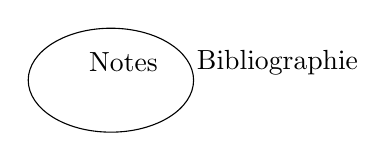
\begin{tikzpicture}
\draw[thin] (0,0) ellipse (1.05cm and .66cm);
\node (n) at (.16,.23) {Notes};
\node[anchor=west,inner sep=1pt] at (1.05,.23) {\deleted{Bibliographie}};
\end{tikzpicture}}
% archive sheet number: 5

\scanpage{11}
% Reused typescript. The type shows through in mirror image from the opposite face.
\[
Z_i=\overline{x_i}\qquad
\begin{array}{c}X_y\\[-2pt]\rotatebox{90}{$\in$}\\[-2pt]x_i\end{array}
\qquad y
\qquad \deg(x_i/y)=\unsure{n_i|n'}
\]
\[
\sum d_i n_i=N
\]

\diagram{\begin{tikzcd}[ampersand replacement=\&,row sep=2em,column sep=2.8em]
X \arrow[r,"f"] \& Y\\
Z_i \arrow[u,phantom,"{\cup\,u_i}" description] \arrow[ur,"{\unsure{f|f_i}}"'] \&
\end{tikzcd}\qquad
\begin{tikzcd}[ampersand replacement=\&,row sep=1.6em,column sep=1.1em]
H^{\unsure{*|r}}(X) \arrow[dr,"u_i^*"'] \& \& H^*(Y) \arrow[ll,bend right=19,draw=gray!55,line width=.2pt] \arrow[ll,bend right=15,"f^*"']\\
\& H^*(Z_i) \arrow[ur,"f_{i*}"'] \&
\end{tikzcd}}

\[
\begin{aligned}
\left(\sum d_i f_{i*}u_i^*\right)f^*
 &=\sum d_i f_{i*}u_i^*f^*\\
 &=\sum d_i\,\tikz[baseline=(a.base)]{\node[inner sep=1pt](a){$f_{i*}f_i^*$};\draw (a.center) ellipse (.48cm and .28cm);}\,n_i\,\mathrm{id}
\end{aligned}
\]
% archive sheet number: 10

\scanpage{16}
\uline{$\overline{\mathrm{XVIII}}$} 1-1

p. 2.

\margin{OK} l \unsure{2\textsuperscript{e}|2} \uline{du} haut

\unsure{Extrait|Expr.} à la \unsure{Ferte|tarte|Ferté} commutent aux images directes.
\margin{\unsure{?}}

\deleted{et ce qui suit \unsure{après sur|après ds|appliquer} les \unsure{catégor.|catégories} dérivées.}
\margin{\unsure{$>$}}

\par\noindent\rule{.9\linewidth}{.2pt}

\margin{\deleted{\unsure{OK}}} l. 9 des bas

\margin{!} pourquoi supposer $X$ réduite à priori \margin{\unsure{3|?}}

\margin{OK} p. 3 l \unsure{7.1|7.|7-8} du haut

embrouillé ---
% archive sheet number: 15

\scanpage{17}
1.4. \mspage{\uuline{14}}

l. 4 du bas

Peut être que le \unsure{Fasceu|Faisceau} $\text{\uuline{Aut}}'(x)$
\unsure{descende|descendu|descend|des automorphismes} de \unsure{s.|$s$|$x$} qui est \uline{dans} $\unsure{\mathrm{pch}|\mathrm{p\,ch}|\mathrm{sch}}(K)$ ?
% archive sheet number: 16

\scanpage{18}
\uline{$\overline{\mathrm{XVIII}}$} -- 1-2.

\margin{OK.} l. 7 \qquad $K_0$ \unsure{entre|autre|attention} \unsure{les|lui} \unsure{mains|mais} $G$
\[
K(K_0,\varphi)=p^*(K_0)+p^*(\varphi)[\unsure{O|\mathcal O}(\unsure{1|\xi|{-}1})]
\]

\par\noindent\rule{.8\linewidth}{.2pt}

\margin{OK} ligne 1 du bas

\unsure{peutêtre|peut être|peut-être} \unsure{métre|mettre} $R^1p_*p^*G$

\par\noindent\hspace*{2em}\rule{.35\linewidth}{.2pt}

\margin{OK} 1.2.2.1 : j'ai mis du \unsure{tem|temps} à comprendre
\unsure{d'abr.|d'abord} \unsure{lire} il \unsure{devien|devient|dernier} \unsure{cd.|c.d.}.

\par\noindent\rule{.9\linewidth}{.2pt}

on \unsure{pourrait|pourrai} faire remarque
\[
\Gamma(S,R^1p_*G)=\frac{H^1(\unsure{P|\mathbb P}(\unsure{E|\mathscr E}),G)}{H^1(S,G)}
\]
\unsure{quand|que|qu'} il y a une section
% archive sheet number: 17

\scanpage{19}
\uline{1-4} \mspage{\tikz[baseline=(p.base)]{\node[inner sep=1pt](p){11};\draw (p.north west) to[out=-100,in=180] (p.south east);\draw ([xshift=-2pt]p.north west) to[out=-100,in=180] ([yshift=-2pt]p.south east);}}

\margin{ok.\\?}
\diagram{$\begin{array}{r||l|l}
\text{l.}&9\ \text{du bas}&\\
&10&?\\
&11&\\
&12&
\end{array}$}
% archive sheet number: 18

\scanpage{20}
\uline{$\overline{\mathrm{XVIII}}$} -- (1.4) \mspage{//2}

l. 1 du haut

on peut \unsure{peutêtre|peut être|peut-être} \unsure{metre|métre|mettre} \unsure{u|n|une} \unsure{ref.|réf.} Mac-Lane

\par\noindent\hspace*{2em}\rule{.25\linewidth}{.2pt}
% archive sheet number: 19

\scanpage{21}
\uline{$\overline{\mathrm{XVIII}}$} -- 1 2

\uuline{p.8}

\margin{OK.} l. 4 du haut

ref \unsure{1.2 7|1.2.7|1.2.1} \unsure{annulée|annulé}
% archive sheet number: 20

\scanpage{22}
\uline{$\overline{\mathrm{XVII}}$} -- 1-2,
\mspage{\tikz[baseline=(p.base)]{\node[inner sep=1pt](p){4};\draw (p.north east) to[out=180,in=90] (p.west) to[out=-90,in=180] (p.south east);}}

(l. 9) du haut

ref. (1.2.2.4)

\margin{OK} mettre (1.2.4.1)

\par\noindent\rule{.83\linewidth}{.25pt}

stop p 4. \uuline{$\overline{\mathrm{XVIII}}$} .1-2.
% archive sheet number: 21

\scanpage{23}
\uline{$\overline{\unsure{\mathrm{VII}|\mathrm{VIII}}}$} .1.2 \mspage{(7}

à \unsure{piéger|piger|préciser}
\[
R^1 f_*(\unsure{G_m|G_{\!u}})
\]

\par\noindent\hspace*{1em}\rule{.65\linewidth}{.2pt}

ligne 0 du bas

\unsure{remplr|rempl.} 1.2.2.1 par (1.2.3) et (1.2.4.1)

\par\noindent\hspace*{1em}\rule{.24\linewidth}{.2pt}
% archive sheet number: 22
